
\chapter{A trip to Jupyter}

\label{programmingEnvironment}
\index{execute}
\index{edit}
\index{language}
\index{environment!programming}
\index{programming environment}
Python is a ridiculously popular \textbf{language} for programming and data
science (currently the third most widely used in the world\footnote{See
\url{https://www.tiobe.com/tiobe-index/}.}) which is one of many reasons we're
using it for this course. The language itself is different from the
\textbf{programming environment} used to write code in it, just as ``English''
is different from ``Microsoft Word'' and ``Google Docs.'' A programming
environment is just a fancy name for a tool or application used to write
programs. At a minimum, it must include a way to \textbf{edit} (write and
revise) code, and a way to \textbf{execute} (run) it.

\index{Jupyter Notebooks}
\index{IDE}
\index{Spyder}
There are many different programming environments data scientists use to write
Python code, just as there are many different word processing apps people use
to write English. The choice largely comes down to personal preference. Some
use full-blown \textbf{IDE}s (``integrated development environments'') like
Spyder or Atom; some use text-based tools like Notepad++ or \texttt{vim}. In
this class, we're going to use the friendly and minimalistic ``\textbf{Jupyter
Notebooks}'' environment since it's appropriate for an intro experience.

\section{Jupyter Notebooks}

\index{cell}
The concept of a Jupyter Notebook is simple. It's just an editable Web page
composed of \textbf{cell}s. Each cell is a little text window you can type in.

There are three kinds of cells in Jupyter Notebooks:

\begin{description}

\label{cell!raw}
\item{\textbf{Raw.}} ``Raw'' is dumb. Never use it.

\label{Markdown}
\label{render}
\label{cell!Markdown}
\item{\textbf{Markdown.}} ``Markdown'' cells are for \textit{English text}, not Python
code. They're mostly used to describe and annotate what you're doing in the
code cells, like a running commentary. You can type plain-ol' text in a
Markdown cell, plus various cutesy formatting adornments like boldface (putting
double-splats (\texttt{**}) around a word or phrase), italics (single splats),
outline headings (prefacing a line with one or more hashtags (like \texttt{\#}
or \texttt{\#\#\#}), and so forth.\footnote{For a complete list of formatting
options, see
\url{https://github.com/adam-p/markdown-here/wiki/Markdown-Cheatsheet}.} When
you type in a Markdown cell, you see the raw text and formatting; to actually get Jupyter to
\textbf{render} your cell and make it pretty, you \textbf{run} the cell by
pressing \textbf{Shift-Enter} while your cursor is inside it.

\label{cell!code}
\item{\textbf{Code.}} The most important cells are ``code'' cells which contain (duh)
code. When executed (again with \textbf{Shift-Enter}) they actually carry out
the Python instructions you have typed in that cell, and display any results.

\end{description}

By the way, a common snafu is to somehow accidentally click in a way that
changes the type of a cell from ``code'' to one of the other types. If you do
this, the Python code in that cell won't execute until you change the type back
to code (more on this below).

\label{cell!type dropdown}
Figure~\ref{fig:jupyterNotebook} shows a Jupyter Notebook hosted by the
\textbf{CoCalc} cloud computing platform, which we'll use this semester. It has
two cells, one Markdown and one code. Note carefully the \textbf{cell-type
dropdown} which is kind of hidden in the middle: it currently reads ``Code''
because the second cell is the one that's highlighted. (If we clicked to
highlight and edit the top cell, that dropdown would change to ``Markdown.'')

\begin{figure}[!h]
\centering
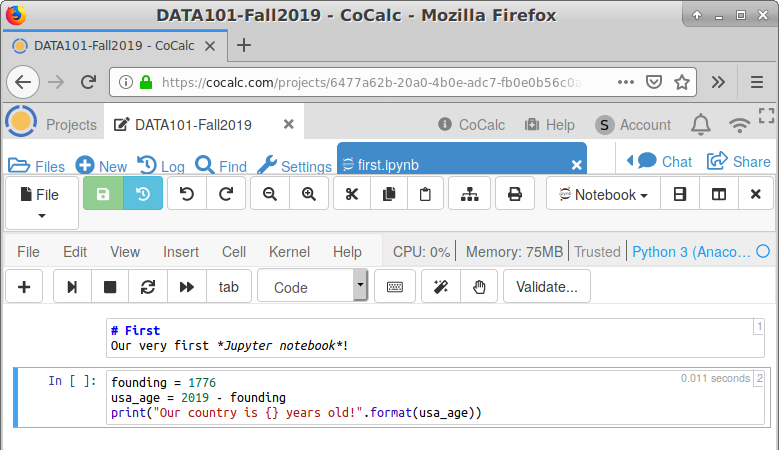
\includegraphics[width=0.9\textwidth]{firstNotebook.png} \\
\bigskip
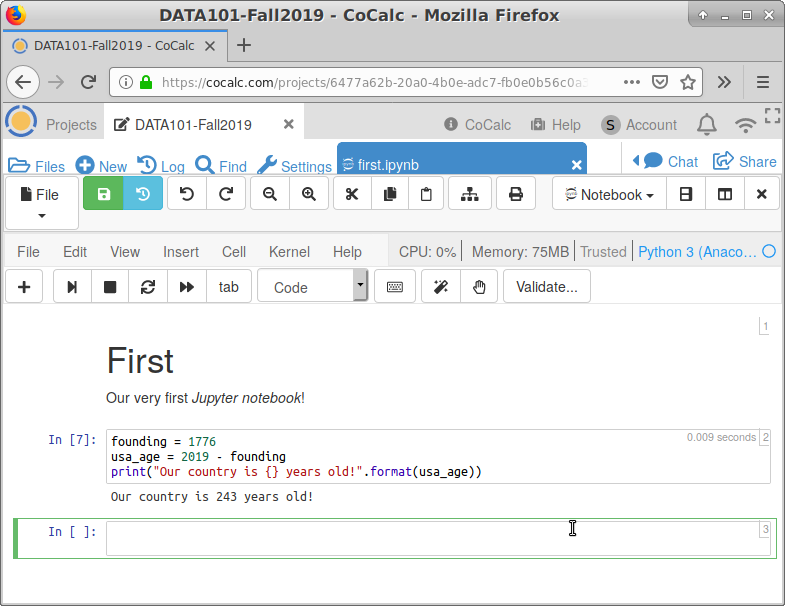
\includegraphics[width=0.9\textwidth]{firstNotebook2.png}
\bigskip
\caption{A Jupyter Notebook with one Markdown cell and one code
cell. In the top pane, the two cells have
been edited but not yet Shift-Enter-ed -- hence the Markdown formatting is
unrendered and the code has not been executed. The bottom pane shows both cells
after they've been Shift-Entere-ed.}
\label{fig:jupyterNotebook}
\end{figure}

\label{code snippet}
\label{snippet}
\label{output}
The top figure shows the two cells before the user has pressed Shift-Enter: all
the Markdown is unrendered (see the literal splats and hashtags) and the code
is just sitting there. After Shift-Enter-ing both cells, the picture changes:
you see the formatted message in the top cell, and the \textbf{output} of the
Python code snippet after it runs. (The latter is easy to miss; stare at that
bottom picture and find the ``\texttt{Our country is 243 years old!}'' message.
That's the ``output.'') We haven't yet covered what that Python code means
(that's the main subject of this book) but you can probably guess a great deal
about what it's doing.

(Btw, you can see that when you Shift-Enter the bottom cell to run the code,
Jupyter also creates a new empty cell at the end of the Notebook for you to
type in. I find this annoying, but whatever.)

\section{Code and output}

Incredibly, that's about it. Everything else in this book is going to concern
what to type in those code cells and how to interpret its output.

From now on, whenever I give example Python code in this book, I'll write it in
a box like this:

\begin{Verbatim}[fontsize=\small,samepage=true,frame=single,framesep=3mm]
founding = 1776
usa_age = 2019 - founding
print("Our country is " + str(usa_age) + " years old!")
\end{Verbatim}

That box means ``this stuff goes in a code cell of a Notebook.''

When I write the corresponding output (\textit{i.e.}, what gets printed on the
page immediately below the code cell when the user highlights the cell and
presses Shift-Enter), I'll write it like this:

\begin{Verbatim}[fontsize=\small,samepage=true,frame=leftline,framesep=5mm,framerule=1mm]
Our country is 243 years old!
\end{Verbatim}

That vertical bar means ``this stuff is the printed result of executing the
code cell.''

Easy. Onward!
